% SASYR 2025 - Template based on:
% samplepaper.tex, a sample chapter demonstrating the
% LLNCS macro package for Springer Computer Science proceedings;
% Version 2.20 of 2017/10/04
%
\documentclass[runningheads]{llncs}
%
\usepackage{graphicx}
\usepackage{lipsum}
\usepackage{url}
\usepackage{siunitx}
\usepackage{amsmath}
\usepackage{subcaption}
\usepackage{booktabs}
\usepackage[labelfont=bf]{caption}
\usepackage{hyperref}
\usepackage{url}
\usepackage{animate}
\usepackage{graphicx}
% Used for displaying a sample figure. If possible, figure files should
% be included in EPS format.
%
% If you use the hyperref package, please uncomment the following line
% to display URLs in blue roman font according to Springer's eBook style:
% \renewcommand\UrlFont{\color{blue}\rmfamily}

\begin{document}
%
\title{Modeling Competing Species in the Presence of a Predator}
%
%\titlerunning{Abbreviated paper title}
% If the paper title is too long for the running head, you can set
% an abbreviated paper title here
%
\author{Grant Lillehei \and
Addison McCarl}

%
\authorrunning{G. Lillehei, A. McCarl}
% First names are abbreviated in the running head.
% If there are more than two authors, 'et al.' is used.
%
\institute{MAT455, Augsburg University, Minneapolis, MN 55414}

%
\maketitle              % typeset the header of the contribution
%
\begin{abstract}
While many different Lotka-Volterra models for inter-species relationships exist, this paper explores a unique situation with logistic growth of prey populations, joint predation, and inter-prey competition. 
As exact solutions cannot be obtained analytically, we utilize five numerical methods and determine RK4 to be the most efficient, requiring the largest step size to achieve errors on the order of $10^{-2}$. 
Under fixed initial conditions in the absence of a predator, we determine the sole stable solution to be the survival of only one of the two prey species. 
We present that a decrease in the birth rate of the surviving species results in a reversal of outcomes, yet find that coexistence is impossible through variation of that parameter alone. 
Further exploration yields a system of inequalities guaranteeing coexistence, which we verify numerically. 
Additionally, we determine that the introduction of a predator enables coexistence under conditions that otherwise result in competitive exclusion, consistent with the ecological principle that joint predation can stabilize prey diversity. 
Comparison to experimental findings reveals that while our model captures qualitative population dynamics, several constant parameters would be realistically interdependent, limiting explicit quantitative applicability.
\end{abstract}
%
%
%
\section{Introduction}
In ecosystems on all scales of life, there exists a wide variety of interspecific relationships, perhaps none more studied than the linked populations of predator and prey. The classic predator-prey dynamic is often modeled by a system of first-order differential equations known as the Lotka-Volterra model.
While the two-species model captures the essential predator-prey oscillation, real ecosystems often involve multiple competing prey with a mutual predator. Understanding how interspecific competition interacts with and without joint predation can reveal insights into ecological modeling with meaningful implications for conservation.
Here, we explore population dynamics between three species in a two-prey, one-predator system, in which prey compete for a limited resource. This variation to the classic model can be described through the following first-order system of differential equations:

\begin{align}
    x' &= \beta_1 x\left(1 - \frac{x}{K_1}\right) - c_1 xy - \alpha_{13} xz, \\
    y' &= \beta_2 y\left(1 - \frac{y}{K_2}\right) - c_2 xy - \alpha_{23} yz, \\
    z' &= \alpha_{31} xz + \alpha_{32} yz - \alpha z
\end{align}

Parameters governing these equations for our model are given in Table ~\ref{tab:constants}, and were designed to reflect plausible population dynamics rather than a specific ecological system. Factors such as differing birth rates and carrying capacities of different orders of magnitude model an inherent difference between the two prey species.

These equations describe changes in population for prey species $x$ and $y$, as well as the predator species $z$. The first terms of Eq. 1 and Eq. 2 model growth in population density from birth rate $\beta_i$, while limited by the individual species carrying capacity $K_i$, modeling logistic growth of each species.

The second term in each respective equation model the natural death rate without predation. Note that each of these terms is multiplied by the current population of the opposing prey. This is meant to simulate competition between species over natural resources. If one prey has a large population density, this limits the resources available to the second prey, and they then die off at higher rates. The final term in Eq. 1 and Eq. 2 represents the death due to predation. This term is directly proportional to predator population density $z$. Each term is multiplied by the current prey population density ($x$ or $y$) so that the death or growth remains proportional. Finally, with the predator model $z'$, the first two terms represent population growth due to predation of $x$ and $y$, respectively. The third term represents some death rate. Again, all three remain proportional to the population as they are multiplied by $z$. 

\begin{table}[htbp]
\centering
\caption{Model Parameters and Initial Conditions}
\label{tab:constants}
\begin{tabular}{@{}lll@{}}
\toprule
\textbf{Parameter} & \textbf{Symbol} & \textbf{Value} \\ \midrule
Birth Rate Species 1                         & $\beta_1$      & $3.15$                  \\
Birth Rate Species 2                         & $\beta_2$      & $2.1$                   \\
Carrying Capacity Species 1                  & $K_1$          & $3.5\times10^{4}$       \\
Carrying Capacity Species 2                  & $K_2$          & $3.5\times10^{5}$       \\
Death Rate Due to Outcompetition Species 1                         & $c_1$          & $3\times10^{-5}$        \\
Death Rate Due to Outcompetition Species 2                         & $c_2$          & $3\times10^{-5}$        \\
Death Rate Due to Predation Species 1                     & $\alpha_{13}$  & $0.15$                  \\
Death Rate Due to Predation Species 2                     & $\alpha_{23}$  & $0.15$                  \\
Predator Growth Rate Attributed to Species 1 & $\alpha_{31}$  & $6\times10^{-5}$        \\
Predator Growth Rate Attributed to Species 2 & $\alpha_{32}$  & $6\times10^{-5}$        \\
Predator Death Rate                          & $\alpha$       & $1.2$                   \\ 
\midrule 
\textbf{Initial Conditions} \\ 
\midrule
Initial Population Density of Prey Species 1 & 
$x_0$ & $3\times10^{3}$ \\
Initial Population Density of Prey Species 2 &
$y_0$ & $3\times10^{3}$ \\
Initial Population Density of Predator &
$z_0$ & $0$ \\
\bottomrule
\end{tabular}
\end{table}

To solve this system of equations, analytical solutions cannot be determined, so we test 5 explicit numerical methods to approximate solutions and analyze states of equilibrium.
Each method has different error convergence and behavior, and we will therefore require varying step sizes for each in order to achieve similar errors. 
The methods with the slowest convergence will require smaller step sizes, and conversely, faster convergence will allow for larger step sizes.
Since no exact solution exists, the error will be approximated by comparison with results from an adaptive method with very low tolerance. 

\section{Explicit Numerical Methods}
\subsection{Euler's Method}
Euler's method is by far the simplest of the 5 explicit approximation 
methods employed in this paper. It uses the current slope at point $x_i$, ($i = 0, \dots, n)$ for n subintervals) which can be found by evaluating one of our differential equations at $f(t_i, x_i)$, We then multiply by our step size h, and add this term to our original point $x_i$ to approximate the point $x_{i+1}$. We then end up with the following formula: $$x_{i+1}=x_i+hf(t_i, x_i)$$

The error approximation for Euler's method is as follows. For an exact 
point $x_i$, it is known that the next point $x_{i+1}$ will at most have an error of $\mathcal{O}(h^2)$. However, this error can accumulate over time. After n iterations, we are left with $n*h^2 = (1/h)*h^2$, meaning our worst-case error is actually represented by $\mathcal{O}(h)$.

\subsection{Improved Euler's Method}
Improved Euler's method is similar, but lends itself to higher 
performance because it uses two different slope approximations to compute the slope at $x_i$. The first approximation, $k_1$, is simply the $f(t_i,x_i)$ computed in the basic Euler's Method. 
Then, $k_2 = hf(t_{i+1}, x_i +hk_1)$. 
This is essentially an approximation of the slope at the next point, $t_{i+1}$. 
The idea is that our look-ahead slope will correct some over/underestimation from our original slope. 
The final equation is as simple as taking a step h with the average of our two slopes: 
$$x_{i+1}=x_i+h(k_1+k_2)$$ 
For an exact $x_i$, we know $x_{i+1}$ to have an error $\mathcal{O}(h^3)$. 
However, as before, we must account for accumulated error. Thus, our final error is $\mathcal{O}(h^2)$.


\subsection{Runge-Kutta Method of Order 4 (RK4)}
The RK4 method uses a combination of 4 different slopes, and takes their weighted average to approximate the slope at $x_{i+1}$ given some $x_i$. Thus, we have $k_1$,$k_2$,$k_3$, and $k_4$ formulated as such: 

\begin{equation}
    \label{k1} k_1=f(t_i,x_i)
\end{equation}
\begin{equation}
    \label{k1} k_2=f(t_i+h/2,x_i+h/2k_1)
\end{equation}
\begin{equation}
    \label{k1} k_3=f(t_i+h/2,x_i+h/2k_2)
\end{equation}
\begin{equation}
    \label{k1} k_4=f(t_i+h,x_i+hk_3)
\end{equation}
Then, a weighted average is taken to compute the slope at $x_{i+1}$:

\begin{equation}
    \label{k1} x_{i+1}=x_i+\frac{h}{6}(k_1+2k_2+2k_3+k_4)
    \end{equation}
This can also be represented with the following Butcher tableau: 
\begin{figure}
    \centering
    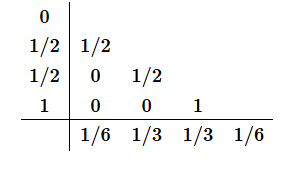
\includegraphics[width=0.5\linewidth]{Figures/rk4tab.png}
    \label{fig:placeholder}
\end{figure}

Whereas the bottom section gives coefficients for each $k_i$, the left section gives the coefficents of h to be added to $t_i$ for each $k_i$, and the diagonal gives coefficents of each h to be multiplied by the corresponding $k_i$ and then subsequently to be added to $t_i$, for each $k_i$. As the name suggests, the error of this method is of order $\mathcal{O}(h^4)$.


\subsection{Runge–Kutta–Fehlberg 45 Adaptive Method (RKF45)}
This adaptive method uses the following Butcher tableau:



\begin{figure}
    \centering
    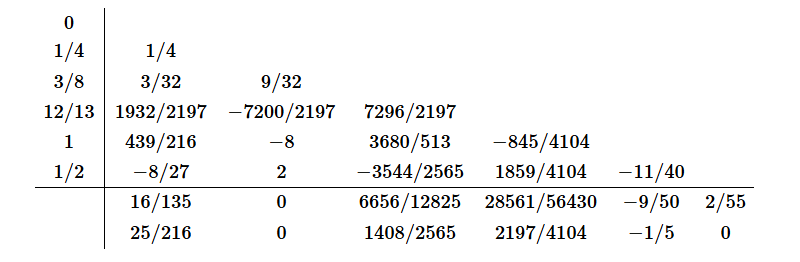
\includegraphics[width=\linewidth]{Figures/rkf45tab.png}
\end{figure}

Whereas the second row produces a method of fifth-order accuracy, while the first produces a method of fourth-order accuracy. At each step, we compute $x_{i+1}$ using both methods, which requires 6 evaluations of $f$. If they produce a difference (an error) outside of our prescribed tolerance, we halve the step size and continue to $x_{i+1}$. 
In addition to an error tolerance, we provide a minimum and maximum h. When we go below the minimum h, we do not halve the h, even if our error tolerance has not been reached. Instead, the method flags the failure and adds it to a tally.  While we are still using an $\mathcal{O}(h^4)$ method, we now dynamically adjust the step size, hopefully resulting in less overall computation to achieve the same error. 

\subsection{Dormand–Prince 45 Adaptive Method (DP45)}
This adaptive method uses the following Butcher tableau:
\begin{figure}
    \centering
    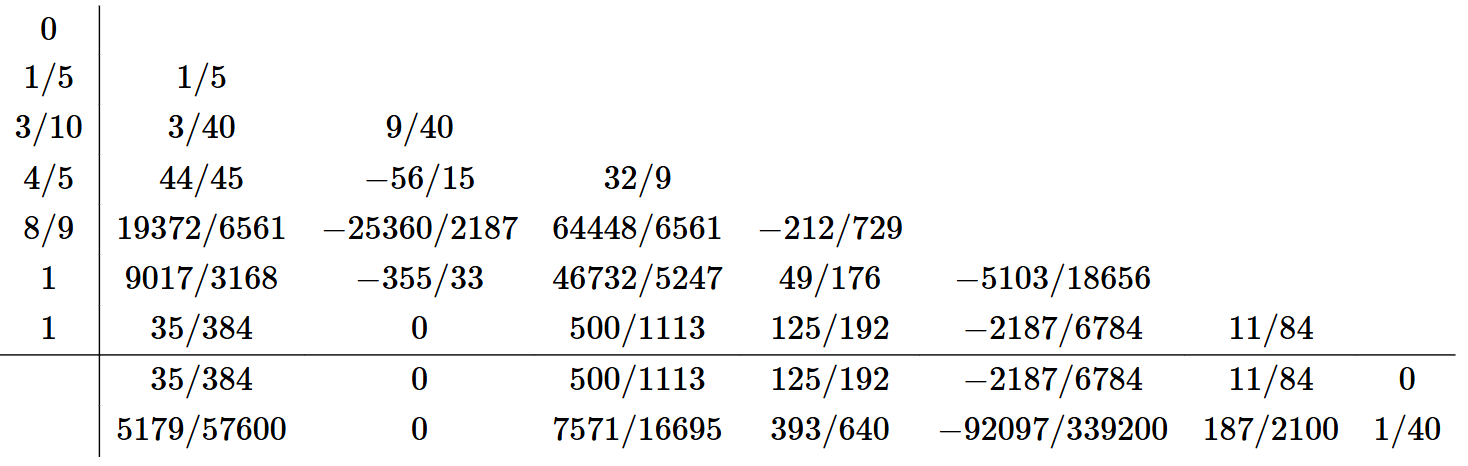
\includegraphics[width=\linewidth]{Figures/dp45tab.png}
\end{figure}

Again, the second row produces a method of fifth-order accuracy, while the first produces a method of fourth-order accuracy. The adaptive aspect of the method works just as in RKF45. Note that the same coefficients are used to compute $k_7$ as are used to compute the fourth-order estimation; this means that this method requires 6 evaluations of $f$ per step, like RKF45. 

\subsection{Determination of a Reference Solution}
Exact solutions cannot be determined analytically for the given system of ODEs, so a method was proposed to compare the error with results from a low-tolerance RKF45 approximation using model parameters from Table ~\ref{tab:constants}. Tolerances for the reference solution are defined within $10^{-16}$ to $10^{-14}$. Comparison to the same model with tolerances between $10^{-12}$ to $10^{-10}$ yields a close idea of reference convergence to the exact solution. Absolute errors between the two tolerances for both species are shown in Figure ~\ref{fig:errordifference}. 

As shown, all errors are $<10^{-9}$, so we consider the reference to approximate the exact solution well. Understanding this limitation, we target an error for all numerical conditions on the order of $10^{-2}$ to ensure the scale of error between our reference and the exact solution does not meaningfully interfere with the calculated error for each method and the reference.

\begin{figure}[!h]
    \centering
    % Adjust [width=0.8\textwidth] if you want it larger or smaller on the page
    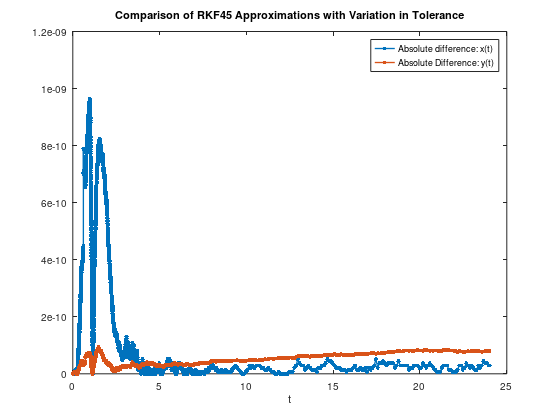
\includegraphics[width=1.0\textwidth, height=0.85\textheight, keepaspectratio]{Figures/errordifference.png}
    \caption{Absolute errors between RKF45 approximations with tolerances between $10^{-16}$ and $10^{-14}$ (reference) and tolerances between $10^{-12}$ and $10^{-10}$.}
    \label{fig:errordifference}
\end{figure}

As RKF45 involves variable step sizes, interpolation is required to calculate the error between methods. 
The reference equation is interpolated using the Octave interp1() function, using a spline method. 
From here, calculating maximum absolute error is as simple as finding the maximum absolute difference between the solution vectors for each population density.

\section{Results}
\subsection{Numerical Method Performance}
We evaluated the efficiency of each numerical approach by varying the step size, $h$ to achieve a comparable absolute error among all methods.

The step size $h$ or tolerances for adaptive methods are picked such that the maximum absolute error is within $10^{-2}$ of our reference equation.

With the initial conditions as described in Table ~\ref{tab:constants}, simulations were run with all 5 models across 24 months. 
All models indicate the extinction of species $x$ with population $y$ limited by its independent-species carrying capacity, $K_2$, as seen in Figure ~\ref{fig:methods}.
All methods but Euler's method converged to a maximum absolute error of $10^{-2}$, as Euler's very poor error convergence of $\mathcal{O}(h)$ would require computational power beyond what was available for this project.
Calculated maximum absolute errors and size of $h$ can be seen in Table ~\ref{tab:performance}.
Tolerances for both RKF45 and DP45 were set between $10^{-3}$ and $10^{-1}$, with step sizes between $10^{-2}$ and $10^{-1}$.

\begin{table}[htbp]
\centering
\caption{Numerical Method Performance}
\label{tab:performance}
\begin{tabular}{@{}lll@{}}
\toprule
\textbf{Numerical Method} & \textbf{Max Absolute Error} & \textbf{Step Size $h$} \\ 
\midrule
Euler & $6.77 \times 10^{0}$ & 1 minute \\
Improved Euler & $1.56 \times 10^{-2}$ & 15 minutes \\
RK4 & $6.819750 \times 10^{-2}$ & 2 days \\
RKF45 & $5.246770 \times 10^{-2}$ & 3.04 hours (average) \\
DP45 & $1.261326 \times 10^{-2}$ & 3.04 hours (average) \\
\bottomrule
\end{tabular}
\end{table}

\begin{figure}[!h]
    \centering
    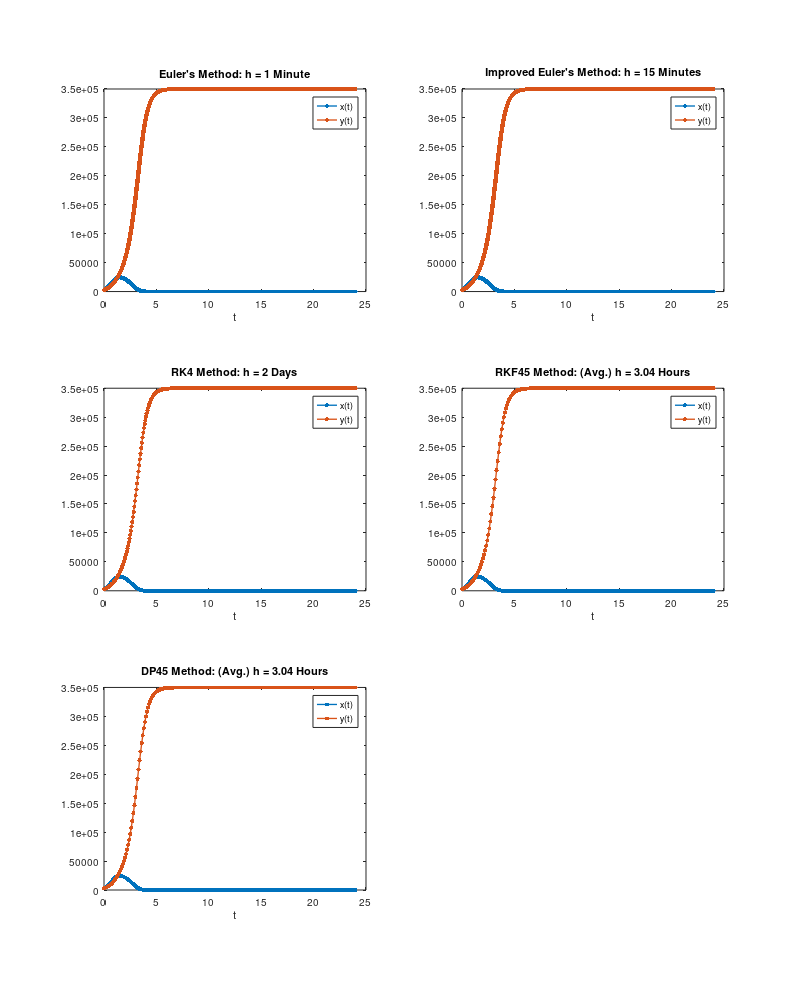
\includegraphics[width=1.0\textwidth, height=0.85\textheight, keepaspectratio]{Figures/methodscomparison.png}
    \caption{Results of all numerical methods with initial conditions from Table ~\ref{tab:constants} from $t = 0$ to $t= 24$ with specified step size $h$.}
    \label{fig:methods}
\end{figure}

From the results, we can determine that our most efficient method here is RK4, with $h = 2$ days. DP45 and RKF45 perform well with $h = 3.04$ hours. For $t<5$, $h$ is relatively large, but as $y$ approaches $k2$, $h$ shrinks dramatically, decreasing the average step size down.


\subsection{Competing Species}
Results of Figure ~\ref{fig:methods} also show that under the given conditions, we reach a stable solution in which $y$ reaches and sustains its independent-species carrying capacity, $K_2$. 
While $x$ initially rises due to its high birth rate, the carrying capacity of $K_1$ is much higher than $K_2$, and therefore its growth is immediately limited. 
The greater increase in $y$ also increases the weight of the term $c_2xy$ in Equation 2, further decreasing the density of the population $x$.

By modifying our initial constants from Table ~\ref{tab:constants}, we can change the surviving population from species $y$ to species $x$. 
One such way is to decrease the birthrate of $y$, $\beta_2$. 
By limiting $\beta_2$, drivers of $x$ outpace those of $y$, while $x \gg y$ reduces population $y$ to extinction.
The value for $\beta_2$ was varied according to binary search to determine the point of bifurcation in which either population wins out, and was determined to a precision of $10^{-15}$ to be:
$$\beta_2 = 1.003294587846742\dots$$
This is not an exact value, and cannot be expressed in terms of other constants, as it depends highly on initial populations and other scenario-specific consequences of the model.
When $\beta_2 < 1.00329\dots$ population $x$ becomes the surviving population, while $\beta_2 > 1.00329\dots$ results in a surviving population $y$.
When exactly equal, numerical methods predict that a metastable solution exists in which both species can coexist, but this is simply an artifact of binary precision.

Alternatively, it is possible for both species to coexist, just not by variation of $\beta_2$ alone. In fact, coexistence can be ensured if the following conditions are met by the initial parameters:
\begin{equation}
\label{eq:stability-conditions}
\begin{aligned}
    \beta_1 &> c_1 K_2 \\
    \beta_2 &> c_2 K_1
\end{aligned}
\end{equation}
This is derived from a 2018 paper \cite{Gavina2018}, with the following equations for their competing species: 

$$
    x' = \beta_1 x \left(1 - \frac{x + \alpha_{12} y}{K_1}\right)
$$

$$
    y' = \beta_2 y \left(1 - \frac{y + \alpha_{21} x}{K_2}\right)
$$

Noticeably, this is extremely similar to our competing species model with their respective $\beta$'s factored out: 

$$
    x' = \beta_1 x \left(1 - \frac{x}{K_1} - \frac{c_1}{\beta_1}y\right)
$$

$$
    y' = \beta_2 y \left(1 - \frac{y}{K_2} - \frac{c_2}{\beta_2}x\right)
$$

Our models then become exactly the same if their $\alpha_{12}$ is set equal to $\frac{c_1 K_1}{\beta_1}$, and if their  $\alpha_{21}$ is set equal to $\frac{c_2 K_2}{\beta_2}$. In their paper they have an inequality that guarantees coexistence: 

$$
    K_1 > \frac{K_2}{\alpha_{21}}
$$

$$
    K_2 > \frac{K_1}{\alpha_{12}}
$$

This inequality becomes the aforementioned inequality~\ref{eq:stability-conditions} applicable to our model when $ \alpha_{12}$ and $\alpha_{21}$ are correctly substituted. Then, coexistence is as simple as choosing values that satisfy our inequality derived from theirs. As is, condition 1 of the inequality is violated: 

$$
    \beta_1 > c_1 K_2 \quad\Rightarrow\quad 3.15 > (3\times10^{-5})(3.5\times10^5) = 10.5
$$

$$
    \beta_2 > c_2 K_1 \quad\Rightarrow\quad 2.1 > (3\times10^{-5})(3.5\times10^4) = 1.05
$$

Hence why coexistence could not be ensured by varying $\beta_2$ alone; the first inequality will always be false regardless of $\beta_2$. Arbitrarily, we chose $\beta_1=12$ to satisfy the first condition, which, as expected, led to coexistence shown in Figure ~\ref{fig:coexistence}.

\begin{figure}[!h]
    \centering
    % Adjust [width=0.8\textwidth] if you want it larger or smaller on the page
    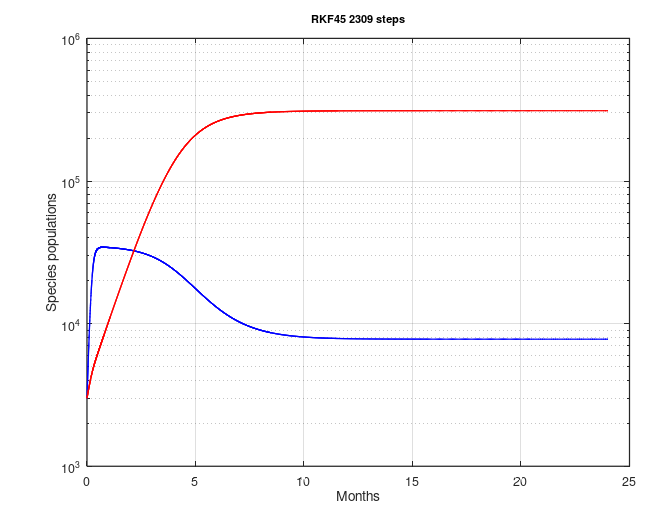
\includegraphics[width=1.0\textwidth, height=0.85\textheight, keepaspectratio]{Figures/coexistnopredator.png}
    \caption{Coexistence of prey populations meeting the inequalities of Equation ~\ref{eq:stability-conditions}.}
    \label{fig:coexistence}
\end{figure}


\subsection{Introducing a Predator}
Upon introducing a predator population, we reset our initial parameters defined in Table ~\ref{tab:constants}, and tested initial predator population densities $z_0=1... 20$, seen in Figure ~\ref{fig:predator}.

\begin{figure}[h]
    \centering
    % {10} is frame rate, {Figures/frame-} is the path + file prefix
    \animategraphics[loop, autoplay, width=0.8\textwidth]{10}{Figures/frame-}{0}{19}
    \caption{Approximation of all three species, with initial predator population densities $z_0=1... 20$.}
    \label{fig:predator}
\end{figure}

Here, it is important to note that the same model with zero predators led to the extinction of one species of prey. For all initial population densities $z_0=1... 20$, long-term behavior indicates convergence to a sole stable equilibrium with survival of all three species. The introduction of a predator population allows the prey to coexist by limiting both populations, minimizing interspecific competition. The more competitive species $x$ can no longer dominate because it is being predated to the degree that it cannot reach a population high enough to outcompete $y$ to extinction.  Not only this, but it is visually apparent that $x$ converges to a significantly lower population than $y$. This is most attributed to $y$'s higher birth rate, which alone was not enough to withstand competition without the presence of a predator. 

\subsection{Limitations of our model}
A Lotka-Volterra model with two species and one predator is well-documented across literature. However, our model is a very specific case. It models logistic growth for each of the prey species, but not for the predator. Consequently, this limits our model such that each prey species is subject to a constant carrying capacity, while the predator has no carrying capacity beyond indirect limitations of populations $x$ and $y$. We assume linear death rates, as well as linear interspecific competition and linear growth of the predator species due to predation. We also assume independent rates of growth for the predator based on which species is being predated. With such a specific case, we will focus on limitations found in literature that are more generally applicable. 

In our first task, we model two competing species with no predators, that is, $z=0$. 
Published research states that oftentimes in these models, one of the species will reach a peak and then subsequently decline to extinction. 
We observed this in our model, but this decline differs from experimental research; in experimental research, the declining species often have one or several reversals before complete extinction\cite{WangerskyLotkaVolterra}.
Our model does not allow for this. 

The presence of a predator can also intensify interspecies competition in the wild, which our model does not account for. This can be true in many cases, as the presence of a predator affects the behavior of prey, but one such case is when predation "restricts habitat use" \cite{KotlerTwoInteractions}. When habitat use is restricted, competition then becomes more intense as there are fewer resources. Perhaps a more sufficient model could somehow involve the rate of predation in the interspecific competition term. 

Also consider that if these two prey species coexist in the same habitat and consume some of the same resources (this is arguably true because there is interspecific competition), their carrying capacities should be somewhat interdependent, meaning not constant. After all, "as prey densities
decline due to predation, the standing crop of resources which they exploit should become more abundant"\cite{KotlerTwoInteractions}. When one of our species becomes extinct or significantly diminished, we should therefore see an increase in resources, which should be followed by an increased carrying capacity for the other species. 

\section{Conclusion}
We approximated a solution to a modified Lotka-Volterra system of differential equations with several different numerical methods. We assessed the error via comparison to a highly converged RKF45 solution, and were able to achieve errors on the order of $10^{-2}$ with every method, except Euler's. Of the methods we implemented, we found RK4 to be the most efficient in terms of average step size. 

We were able to dictate which species survived by varying only $\beta_2$, and found a threshold value that produced the illusion of coexistence to binary precision. We derived an inequality system (Eq. ~\ref{eq:stability-conditions}) which guarantees coexistence, then satisfied it through variation in $\beta_1$. We also found that the introduction of a predator allowed coexistence under our initial parameterization due to the limiting of competition, whereas in the absence of a predator, one prey species became extinct. This result is consistent with the broader ecological principle that a shared predator can mediate competition, effectively acting as a stabilizing force on prey diversity.

Comparison to experimental and biological findings revealed several limitations of our model. Several parameters, particularly carrying capacities and competition coefficients, would realistically be interdependent in an ecological system, limiting the quantitative applicability of our results.
Future work could incorporate dynamic capacities or prey responses to predation to model the system more accurately. 
Regardless, the qualitative dynamics presented here align with published ecological findings and demonstrate the utility of numerical methods in exploring systems without analytical solutions. 

\section{Author Contributions}
Both authors contributed equally to this work. 
Both authors created their own implementation of each method to solve the model and confirmed their solutions were working correctly. 
Grant developed an interpolation method in order to use RKF45 as a reference solution, and assessed each method against it.
Addison researched the limitations of mathematical modeling of biological systems and assessed our specific model. 
Grant determined the threshold for $\beta_2$ through binary search.
Addison completed the write-up of the secondary tasks with joint input from Grant. 
Addison completed an initial conclusion and abstract, polished by Grant. 
Grant uploaded his work to and managed the cited GitLab directory. 
All work was split equitably, often with an Agile approach, and both authors take equal credit for the final submission.

\bibliographystyle{ieeetr}
\bibliography{refs}

\section*{Code Availability}
The source code is available at the following repository: \url{https://gitlab.com/lilleheg/competing-species/}

\end{document}
